Model uczenia maszynowego jaki został wykorzystany w testach to sieć neuronowa.

Do testów stworzone zostało kilka modeli sieci neuronowych,
wytrenowanych na rysunkach grafów stworzonych za pomocą skryptów R.
Implementacja została wykonana biblioteką TensorFlow oraz Keras w języku Python.
Modele są w stanie rozpoznawać rysunki grafów i przypisywać im odpowiednie klasy.
Celem było również przetestowanie modeli na rzeczywistych zdjęciach,
zawierających wzorce przypominające grafy, bądź rysunkach grafów narysowanych ręcznie.

Stworzone zostały 3 modele:
- wytrenowany na danych ze stałą liczbą wierchołków
- wytrenowany na danych ze stałą liczbą wierchołków oraz walidacją krzyżową
- wytrenowany na danych ze zmienną liczbą wierzchołków

\subsection{Generacja danych}
Dane wygenerowane zostały przy pomocy skryptu stworoznego w języku R oraz biblioteki igraph.
Skrypt został zaprojektowany funkcyjnie, by osiągnąć możliwie największą automatyzację testów.
Rysunki grafów tworzone są o wielkości 800x600 pikseli, na białym tle, z wierzchołkami w kolorze pomarańczowym,
bez jakichkolwiek oznaczeń wierzchołków oraz zapisywane są w odpowiednich katalogach, odpowiadających klasie grafu.
Przygotowane zostały funkcje tworzące ścieżki, grafy cykliczne, grafy pełne, grary spójne, grafy dwudzielne oraz puste.
W każdej z funkcji możliwy jest wybór liczby generowanych grafów, liczba wierzchołków grafu
oraz współczynnik odpowiadający za zakrzywienie krawędzi na rysunkach.

\subsection{Opis skryptu}
Obrazy z katalogów roboczych 

\subsection{Model}
Na początku dane zostały przygotowane ze zbioru obrazów, znajdującego się w katalogu lokalnym.
Dokonany został podział na zbiory treningowe i walidacyjne.
Dla każdego przejścia walidacji krzyżowej, dane zostały podzielone inaczej.
Po wczytaniu danych, zostały przeskalowane i przeskztałcone do odcieni szarości.

Model sieci neuronowej został zdefiniowany jako sekwencyjny stos warstw.
Pierwsza warstwa to warstwa Rescaling, która normalizuje wartości pikseli do zakresu [0, 1].
Następne trzy warstwy to Conv2D z wybraną liczbą filtrów, z których każda jest poprzedzona warstwą MaxPooling2D.
Warstwy konwolucyjne używają różnych funkcji akytwacji, np. ReLU.
Po warstwach konwolucyjnych znajduje się warstwa Flatten, która przekształca mapy cech 2D w wektor 1D.
Następnie dodana jest w pełni połączona (Dense) warstwa z wybraną liczbą jednostek
i wybraną funkcją aktywacji, wraz z warstwą dropout.
Zastosowana jest tam również regularyzacja L2 (zmniejszanie wag) z ustaloną siłą regularyzacji wynoszącą.
Warstwa wyjściowa zawiera tyle jednostek, ile występuje klas.
Zależnie od danego testu, może być to różna liczba.

\subsection{Wyniki}
Najlepsze wyniki zostały uzyskane przy użyciu modelu sieci neuronowej z walidacją krzyżową K-Fold z liczbą podziałów równą 5.
Dla wszystkich warstw wybrana została funkcja aktywacji ReLU.
W przypadku warstw konwolucyjnych, wybrano 32 filtry, a dla warstwy w pełni połączonej zastosowano 128 jednostek.
Regularyzacja została zastosowana z siłą 0,01, a współczynnik dropout - 0,2.

\subsubsection{Model podstawowy}

\begin{figure}[ht]
	\centering
	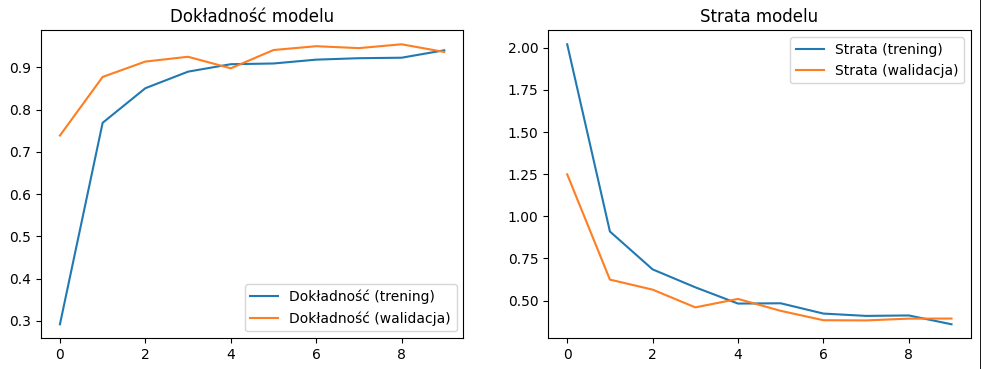
\includegraphics[height=5.5cm]{partials/images/tests/v2.png}
	\caption{Wyniki testów dla modelu podstawowego}
\label{Fig:GraphUndirected}
\end{figure}
\FloatBarrier

\subsubsection{Model z walidacją krzyżową}

\begin{figure}[ht]
	\centering
	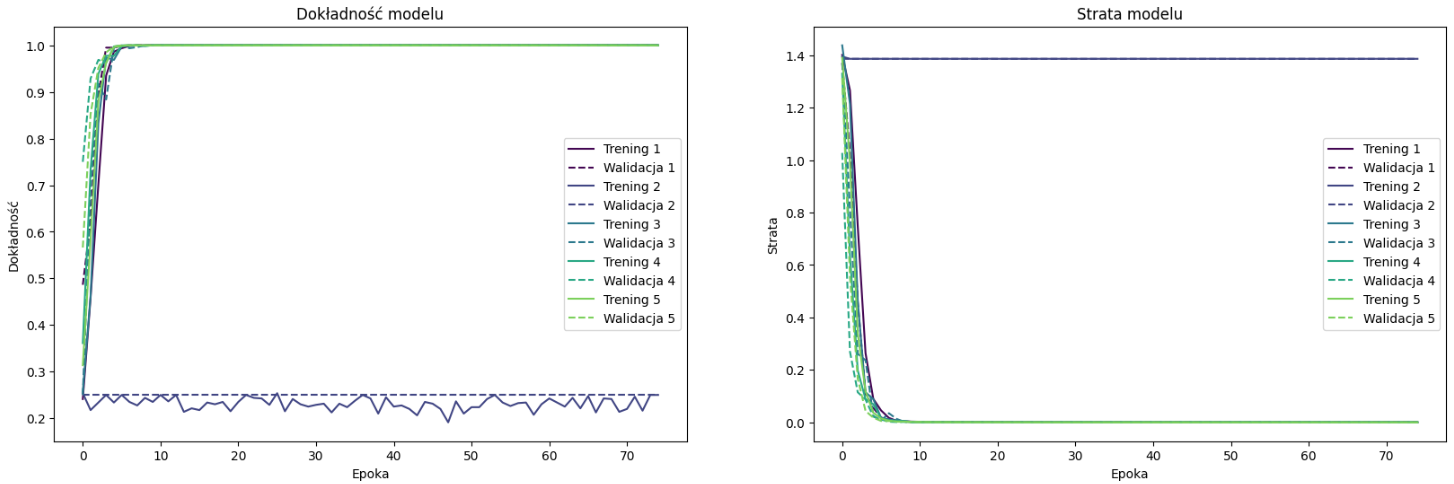
\includegraphics[height=5cm]{partials/images/tests/v2_crossvalid.png}
	\caption{Wyniki testów dla modelu z walidacją krzyżową}
\label{Fig:GraphUndirected}
\end{figure}
\FloatBarrier

\subsubsection{Model ze zmienną liczbą wierzchołków}
\begin{figure}[ht]
	\centering
	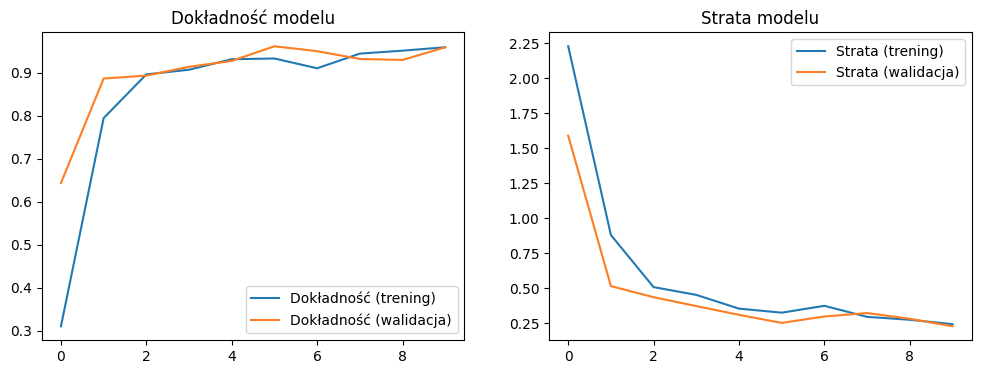
\includegraphics[height=5.5cm]{partials/images/tests/v2_multiple_edges.png}
	\caption{Wyniki testów dla modelu ze zmienną liczbą wierzchołków}
\label{Fig:GraphUndirected}
\end{figure}
\FloatBarrier

\subsubsection{Model ze zmienną liczbą wierzchołków i walidacją krzyżową}

\begin{figure}[ht]
	\centering
	% \includegraphics[height=5.5cm]{partials/images/tests/v2_multiple_edges_crossvalid.png}
	\caption{Wyniki testów dla modelu ze zmienną liczbą wierzchołków i walidacją krzyżową}
\label{Fig:GraphUndirected}
\end{figure}
\FloatBarrier

\subsection{Wnioski}
Przy modelach uczonych na danych zawierających rysunki grafów dwudzielnych, ciężko było wyciągnąć poprawne wnioski.
Działo się tak ze względu na podobieństwo grafów dwudzielnych do innych typów grafów. 

W przypadku uczenia modeli z wykorzystaniem grafów pełnych, najczęściej dominowały one cały zbiór danych,
przez co modele w kolejnych testach klasyfikowały większość testowych grafów rysowanych odręcznie jako właśnie grafy pełne.

Testy z wykorzystaniem stałej liczby wierzchołków grafów okazały się mniej owocne niż testy z rysunkami grafów
o zmiennej liczbie wierchołków.